\documentclass{beamer}
\usepackage{default}

% Language
\usepackage[portuguese]{babel}
\usepackage[utf8]{inputenc}
\usepackage{algpseudocode}
%\usepackage{algorithm}

% Graphics
\usepackage{svg}

% Code highlighting
\usepackage[cache=false]{minted}

\newmintedfile[inputcppcode]{c++}{linenos=false,mathescape,tabsize=4,frame=none}
\newcommand{\inputcpp}[2]{
\begin{block}{#1}
    \inputcppcode{codes/#2.cpp}
\end{block}
}

\newcommand{\titleslide}[1]{
    \begin{frame}
    \begin{center}
    \Huge #1
    \end{center}
    \end{frame}
}

% Theme
\usetheme{Warsaw}


\begin{document}

\title{Buscas e Caminhos Mínimos em Grafos}
\subtitle{}
\author{Roberto Sales}
\date{}
\maketitle

\begin{frame}{Buscas em grafos}
    \begin{itemize}
        \item Permitem responder perguntas sobre conectividade
        \begin{enumerate}
            \item O vértice $u$ está conectado ao vértice $v$ / existe caminho entre $u$ e $v$.
            \item É possível transitar entre qualquer par de vértices $(u, v)$ num dado grafo direcionado $G$? (problema da conectividade forte)
            \item Existe a garantia de que, se uma aresta for removida, o grafo continuará conexo? (problema das pontes)
        \end{enumerate}
    \end{itemize}
\end{frame}

\begin{frame}{Buscas em grafos}
    \begin{itemize}
        \item Permitem responder perguntas sobre propriedades do grafo
        \begin{enumerate}
            \item O grafo não-direcionado $G$ contém ciclos?
            \item O grafo $G$ é um grafo bipartido?
        \end{enumerate}
    \end{itemize}
    
    \begin{itemize}
        \item Permitem resolver problemas de otimização
        \begin{enumerate}
            \item Caminhos mais curtos num grafo
            \item Caminhos mais longos em alguns grafos com características específicas
            \item Caminho entre dois vértices $u, v$ tal que a aresta de menor capacidade (gargalo) é a maior possível
        \end{enumerate}
    \end{itemize}
\end{frame}

\titleslide{Busca em Profundidade}

\begin{frame}{Busca em Profundidade (DFS)}
    \begin{block}{Estratégia}
        Visitar os vértices do grafo de forma recursiva, seguindo sempre pelo próximo vértice não explorado, até que não seja mais possível continuar. Em geral, visita todo vértice e processa toda aresta no máximo uma vez e, portanto, pára. \\~\\
        
        \textbf{Complexidade:} $O(|V|+|E|)$
    \end{block}
\end{frame}

\begin{frame}{Busca em Profundidade}
    \inputcpp{DFS clássica}{dfs}
\end{frame}

\begin{frame}{Busca em Profundidade (DFS)}
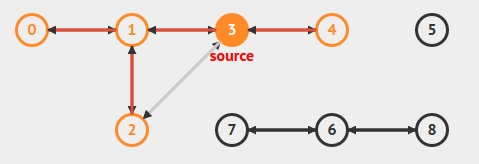
\includegraphics[width=\linewidth]{img/dfs1.jpg}
\end{frame}

\begin{frame}{Busca em Profundidade (DFS)}
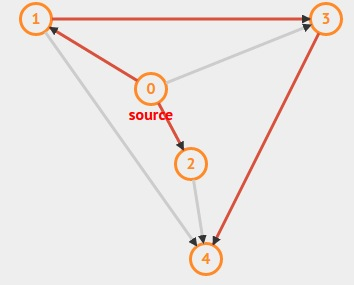
\includegraphics[width=\linewidth]{img/dfs2.jpg}
\end{frame}


\begin{frame}{Aplicações da DFS}
\begin{block}{Não resolve}
    \begin{itemize}
        \item Problemas de caminhos mínimos em grafos gerais
        \item Problemas de caminhos mais longos em grafos gerais
    \end{itemize}
\end{block}

\begin{block}{Resolve}
    \begin{itemize}
        \item Bicolorir um grafo
        \item Checar conectividade, contar componentes conexas
        \item Otimizações em árvores
    \end{itemize}
\end{block}

\begin{block}{Variações}
    \begin{itemize}
        \item Circuito euleriano
        \item Caminhos aumentantes (fluxos)
        \item Componentes biconexas, pontes e pontos de articulação
        \item Componentes fortemente conexas
    \end{itemize}
\end{block}
\end{frame}

\begin{frame}{Variações}
\inputcpp{Bicoloração}{coloring}
\end{frame}

\titleslide{Busca em Largura}

\begin{frame}{Busca em Largura (BFS)}
\begin{block}{Estratégia}
Ao invés de visitar os vértices de forma recursiva, iremos visitá-los em camadas. Em termos de implementação, a única mudança é que deixaremos de usar uma pilha implícita (recursão) em favor de uma fila.
\end{block}
\end{frame}

\begin{frame}{BFS vs. DFS}
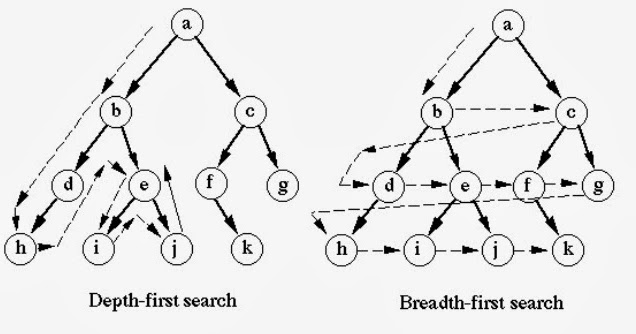
\includegraphics[width=\linewidth]{img/dfsbfs.jpg}
\end{frame}

\begin{frame}{Busca em Largura (BFS)}
\inputcpp{BFS}{bfs}
\end{frame}

\begin{frame}{Busca em Largura (BFS)}
\inputcpp{BFS (caminhos mínimos)}{bfs2}
\end{frame}

\begin{frame}{BFS vs. DFS}
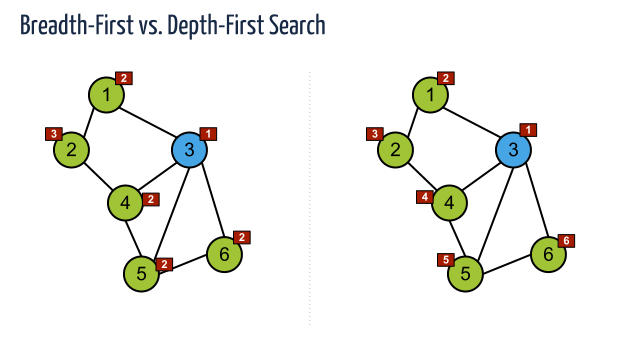
\includegraphics[width=\linewidth]{img/dfsbfs2.png}
\end{frame}

\begin{frame}
\begin{block}{Curiosidades}
Um grafo não precisa estar explicitamente representado na memória para que um algoritmo de busca ou de caminhos mínimos seja executado nele.
\end{block}

\begin{block}{Exemplos}
\begin{itemize}
    \item Problema de caminho mais curto num labirinto (BFS)
    \item Ladrilhos (Regional - Maratona de Programação 2016) (DFS/BFS)
    \item Mania de Par (Regional - Maratona de Programação 2015) (dijkstra)
    \item Contêineres (Regional - Maratona de Programação 2016) (dijkstra)
\end{itemize}
\end{block}

Qualquer coisa que expresse relações pode ser um grafo, fique atento!
\end{frame}

\titleslide{Dijkstra}

\begin{frame}{Dijsktra}
\begin{block}{Motivação}
    Computar caminhos mínimos a partir de um vértice $u$ em um grafo com arestas de custo \textbf{não-negativo}.
\end{block}

\begin{block}{Subestrutura ótima dos caminhos mínimos}
    Para todo caminho $u$-$v$-$w$, onde $(v, w)$ é uma aresta do grafo em questão, se $u$-$v$-$w$ é um caminho mínimo, então $u$-$v$ é um caminho mínimo.
\end{block}

\end{frame}


\begin{frame}
\begin{algorithmic}[1]
    \Procedure{Dijkstra}{$V, E, s$}
        \ForAll {$u \in V \setminus \{s\}$}
            \State $d_u = oo$
        \EndFor
        
        \State $d_s = 0$
        \State $S = \emptyset$
        \While{$S \neq V$}
            \State extract $u \notin S$ such that $d_u$ is minimum
            \State $S = S \cup \{u\}$
            \For{$v$ adjacent to $u$} \Comment{relaxing step}
                \If{$d_u + w(u,v) < d_v$}
                    \State $d_v = d_u + w(u,v)$
                \EndIf
            \EndFor
        \EndWhile
    \EndProcedure
\end{algorithmic}
\end{frame}

\begin{frame}{Desafios}

\begin{block}{XOR Equations}
    Dadas $n$ variáveis booleanas $x_1, x_2, \cdots, x_n$ e $m$ equações na forma $x_i \oplus x_j = z$, onde $z \in \{0, 1\}$, determine se o sistema tem uma solução. Em caso positivo, descubra uma.
\end{block}

\begin{block}{Sequência Lexicograficamente Máxima}
    Dada uma sequência de inteiros $s_1, s_2, \cdots, s_n$ e um conjunto de operações válidas $X$, determine a maior sequência lexicograficamente que é possível obter usando um número finito de operações. \\~\\
    
    O conjunto $X$ tem $m$ pares na forma $(i, j)$. Tal par descreve uma operação de troca entre as posições $i$ e $j$ da sequência.
\end{block}
\end{frame}

\end{document}
